\chapter{モジュール生産状況の解析}

データベースシステムを使って、モジュール生産状況の解析を行うことができる。
モジュールの組み立て工程は各組み立て機関のローカルデータベース上に記録され、組み立て工程ごとに中央データベースへ同期される。
そのため全モジュールの現在工程を中央データベース上で取得できることができ、この情報を用いて世界的な生産状況の解析を行うことができる。
現在は生産は行われていないが、想定している解析結果のイメージを図\ref{production_analysis}に示す。

\begin{figure}[bpt]\centering
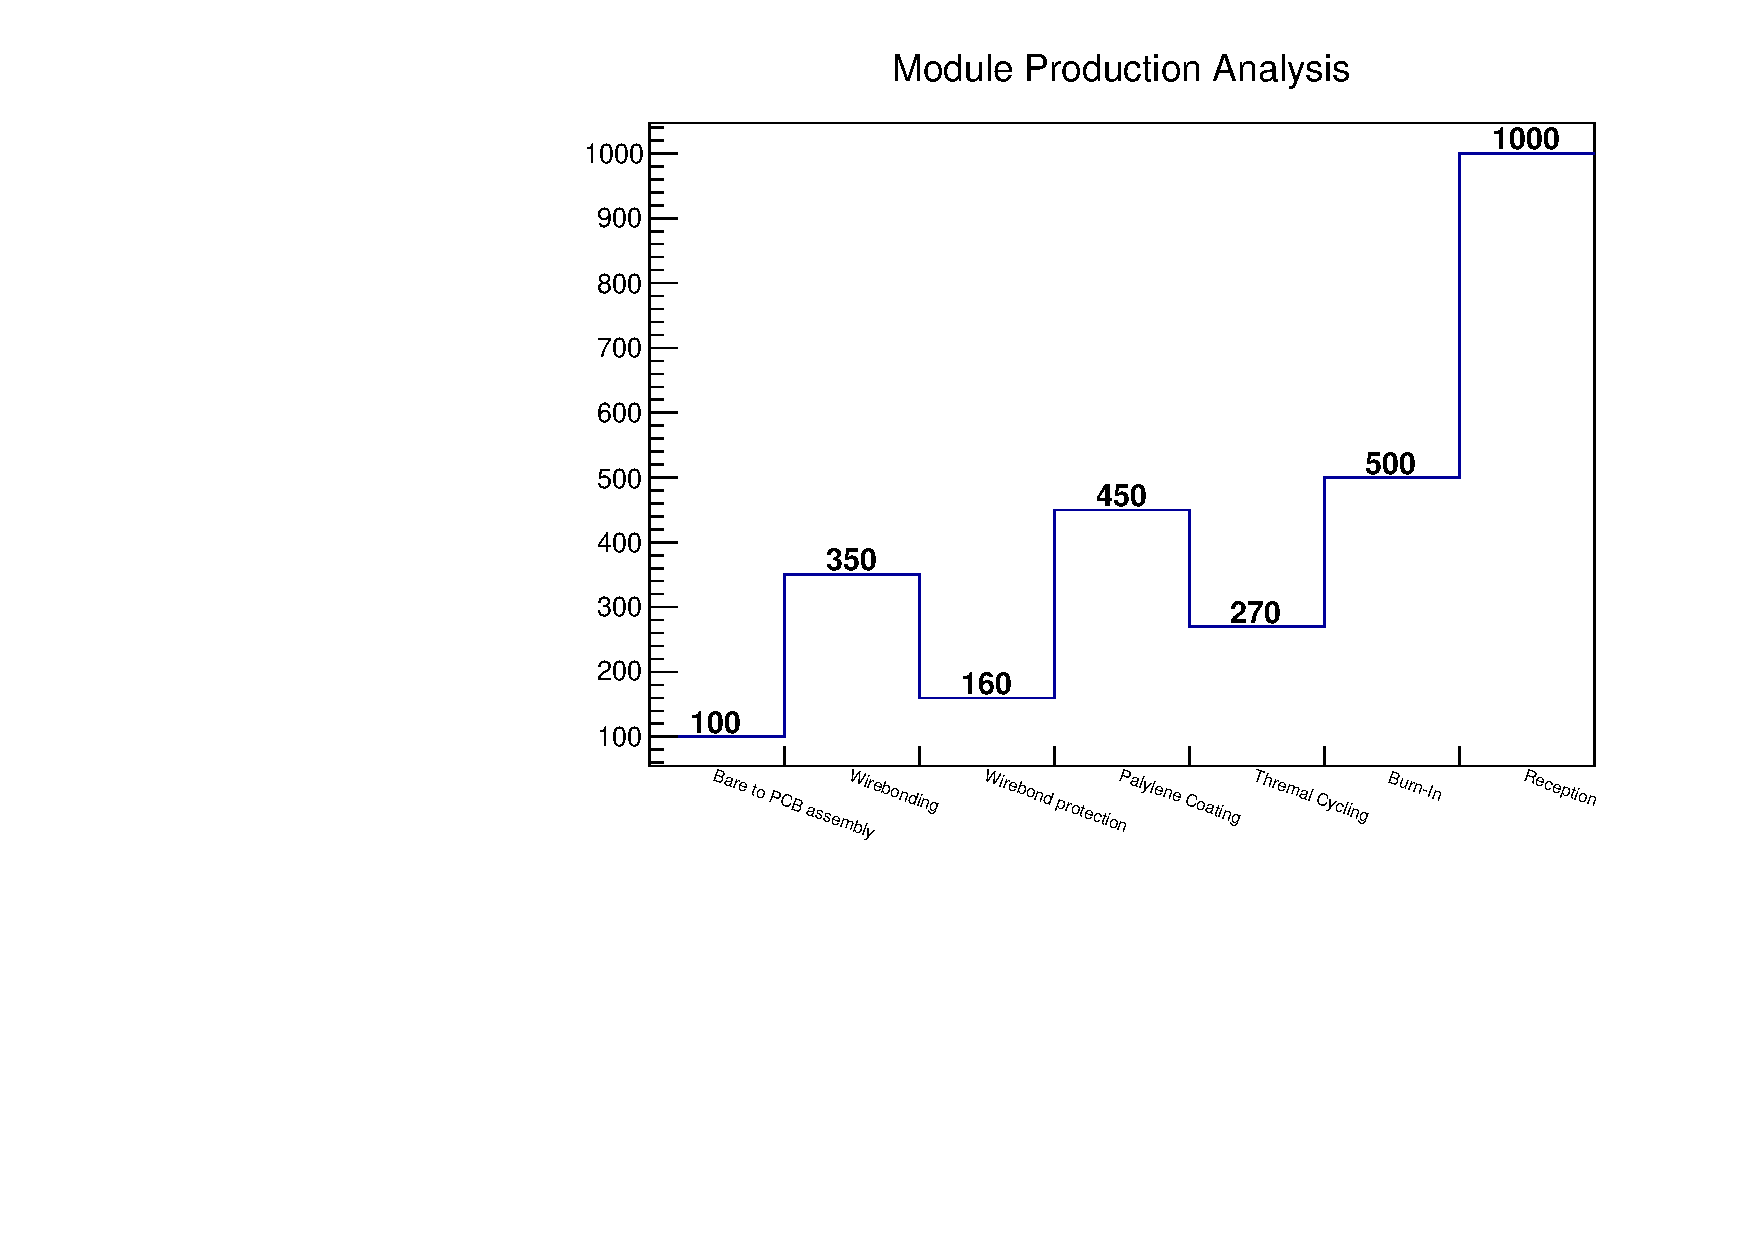
\includegraphics[width=8cm,angle=270]{./production_analysis.pdf}
\caption[生産時のモジュール組み立て状況解析の例]{生産時のモジュール組み立て状況解析の例。ローカルデータベースにて組み立て工程は管理され、工程毎に中央データベースに同期されるため、生産時には全モジュールの現工程を中央データベースで取得できる。図の例ように各段階におけるモジュール数を見ることで生産状況の確認ができる。さらにある期間ごとに工程を取得することで生産レートなども計算することができ、今後の生産計画やモジュール選別の参考とすることができる。}
\label{production_analysis}
\end{figure}

生産数や生産レートのモニタリングを行うことで、今後の生産計画や問題解決に役立てることが可能である。

